% GNUPLOT: LaTeX picture with Postscript
\begingroup
  \fontfamily{ptm}%
  \selectfont
  \makeatletter
  \providecommand\color[2][]{%
    \GenericError{(gnuplot) \space\space\space\@spaces}{%
      Package color not loaded in conjunction with
      terminal option `colourtext'%
    }{See the gnuplot documentation for explanation.%
    }{Either use 'blacktext' in gnuplot or load the package
      color.sty in LaTeX.}%
    \renewcommand\color[2][]{}%
  }%
  \providecommand\includegraphics[2][]{%
    \GenericError{(gnuplot) \space\space\space\@spaces}{%
      Package graphicx or graphics not loaded%
    }{See the gnuplot documentation for explanation.%
    }{The gnuplot epslatex terminal needs graphicx.sty or graphics.sty.}%
    \renewcommand\includegraphics[2][]{}%
  }%
  \providecommand\rotatebox[2]{#2}%
  \@ifundefined{ifGPcolor}{%
    \newif\ifGPcolor
    \GPcolortrue
  }{}%
  \@ifundefined{ifGPblacktext}{%
    \newif\ifGPblacktext
    \GPblacktexttrue
  }{}%
  % define a \g@addto@macro without @ in the name:
  \let\gplgaddtomacro\g@addto@macro
  % define empty templates for all commands taking text:
  \gdef\gplbacktext{}%
  \gdef\gplfronttext{}%
  \makeatother
  \ifGPblacktext
    % no textcolor at all
    \def\colorrgb#1{}%
    \def\colorgray#1{}%
  \else
    % gray or color?
    \ifGPcolor
      \def\colorrgb#1{\color[rgb]{#1}}%
      \def\colorgray#1{\color[gray]{#1}}%
      \expandafter\def\csname LTw\endcsname{\color{white}}%
      \expandafter\def\csname LTb\endcsname{\color{black}}%
      \expandafter\def\csname LTa\endcsname{\color{black}}%
      \expandafter\def\csname LT0\endcsname{\color[rgb]{1,0,0}}%
      \expandafter\def\csname LT1\endcsname{\color[rgb]{0,1,0}}%
      \expandafter\def\csname LT2\endcsname{\color[rgb]{0,0,1}}%
      \expandafter\def\csname LT3\endcsname{\color[rgb]{1,0,1}}%
      \expandafter\def\csname LT4\endcsname{\color[rgb]{0,1,1}}%
      \expandafter\def\csname LT5\endcsname{\color[rgb]{1,1,0}}%
      \expandafter\def\csname LT6\endcsname{\color[rgb]{0,0,0}}%
      \expandafter\def\csname LT7\endcsname{\color[rgb]{1,0.3,0}}%
      \expandafter\def\csname LT8\endcsname{\color[rgb]{0.5,0.5,0.5}}%
    \else
      % gray
      \def\colorrgb#1{\color{black}}%
      \def\colorgray#1{\color[gray]{#1}}%
      \expandafter\def\csname LTw\endcsname{\color{white}}%
      \expandafter\def\csname LTb\endcsname{\color{black}}%
      \expandafter\def\csname LTa\endcsname{\color{black}}%
      \expandafter\def\csname LT0\endcsname{\color{black}}%
      \expandafter\def\csname LT1\endcsname{\color{black}}%
      \expandafter\def\csname LT2\endcsname{\color{black}}%
      \expandafter\def\csname LT3\endcsname{\color{black}}%
      \expandafter\def\csname LT4\endcsname{\color{black}}%
      \expandafter\def\csname LT5\endcsname{\color{black}}%
      \expandafter\def\csname LT6\endcsname{\color{black}}%
      \expandafter\def\csname LT7\endcsname{\color{black}}%
      \expandafter\def\csname LT8\endcsname{\color{black}}%
    \fi
  \fi
    \setlength{\unitlength}{0.0500bp}%
    \ifx\gptboxheight\undefined%
      \newlength{\gptboxheight}%
      \newlength{\gptboxwidth}%
      \newsavebox{\gptboxtext}%
    \fi%
    \setlength{\fboxrule}{0.5pt}%
    \setlength{\fboxsep}{1pt}%
    \definecolor{tbcol}{rgb}{1,1,1}%
\begin{picture}(7200.00,4320.00)%
    \gplgaddtomacro\gplbacktext{%
      \csname LTb\endcsname%%
      \put(166,3526){\makebox(0,0)[r]{\strut{}\tiny }}%
      \csname LTb\endcsname%%
      \put(166,3770){\makebox(0,0)[r]{\strut{}\tiny }}%
      \csname LTb\endcsname%%
      \put(166,4014){\makebox(0,0)[r]{\strut{}\tiny }}%
      \csname LTb\endcsname%%
      \put(1157,3311){\makebox(0,0){\strut{}\tiny 0.1}}%
      \csname LTb\endcsname%%
      \put(2302,3311){\makebox(0,0){\strut{}\tiny 1}}%
      \csname LTb\endcsname%%
      \put(3447,3311){\makebox(0,0){\strut{}\tiny 10}}%
    }%
    \gplgaddtomacro\gplfronttext{%
      \csname LTb\endcsname%%
      \put(3080,4134){\makebox(0,0)[r]{\strut{}\tiny size bin 1}}%
    }%
    \gplgaddtomacro\gplbacktext{%
      \csname LTb\endcsname%%
      \put(3756,3526){\makebox(0,0)[r]{\strut{}\tiny }}%
      \csname LTb\endcsname%%
      \put(3756,3770){\makebox(0,0)[r]{\strut{}\tiny }}%
      \csname LTb\endcsname%%
      \put(3756,4014){\makebox(0,0)[r]{\strut{}\tiny }}%
      \csname LTb\endcsname%%
      \put(4747,3311){\makebox(0,0){\strut{}\tiny 0.1}}%
      \csname LTb\endcsname%%
      \put(5892,3311){\makebox(0,0){\strut{}\tiny 1}}%
      \csname LTb\endcsname%%
      \put(7037,3311){\makebox(0,0){\strut{}\tiny 10}}%
    }%
    \gplgaddtomacro\gplfronttext{%
      \csname LTb\endcsname%%
      \put(6670,4134){\makebox(0,0)[r]{\strut{}\tiny size bin 5}}%
    }%
    \gplgaddtomacro\gplbacktext{%
      \csname LTb\endcsname%%
      \put(166,2451){\makebox(0,0)[r]{\strut{}\tiny }}%
      \csname LTb\endcsname%%
      \put(166,2695){\makebox(0,0)[r]{\strut{}\tiny }}%
      \csname LTb\endcsname%%
      \put(166,2939){\makebox(0,0)[r]{\strut{}\tiny }}%
      \csname LTb\endcsname%%
      \put(1157,2236){\makebox(0,0){\strut{}\tiny 0.1}}%
      \csname LTb\endcsname%%
      \put(2302,2236){\makebox(0,0){\strut{}\tiny 1}}%
      \csname LTb\endcsname%%
      \put(3447,2236){\makebox(0,0){\strut{}\tiny 10}}%
    }%
    \gplgaddtomacro\gplfronttext{%
      \csname LTb\endcsname%%
      \put(3080,3059){\makebox(0,0)[r]{\strut{}\tiny size bin 8}}%
    }%
    \gplgaddtomacro\gplbacktext{%
      \csname LTb\endcsname%%
      \put(3756,2451){\makebox(0,0)[r]{\strut{}\tiny }}%
      \csname LTb\endcsname%%
      \put(3756,2695){\makebox(0,0)[r]{\strut{}\tiny }}%
      \csname LTb\endcsname%%
      \put(3756,2939){\makebox(0,0)[r]{\strut{}\tiny }}%
      \csname LTb\endcsname%%
      \put(4747,2236){\makebox(0,0){\strut{}\tiny 0.1}}%
      \csname LTb\endcsname%%
      \put(5892,2236){\makebox(0,0){\strut{}\tiny 1}}%
      \csname LTb\endcsname%%
      \put(7037,2236){\makebox(0,0){\strut{}\tiny 10}}%
    }%
    \gplgaddtomacro\gplfronttext{%
      \csname LTb\endcsname%%
      \put(6670,3059){\makebox(0,0)[r]{\strut{}\tiny size bin 9}}%
    }%
    \gplgaddtomacro\gplbacktext{%
      \csname LTb\endcsname%%
      \put(166,1376){\makebox(0,0)[r]{\strut{}\tiny }}%
      \csname LTb\endcsname%%
      \put(166,1620){\makebox(0,0)[r]{\strut{}\tiny }}%
      \csname LTb\endcsname%%
      \put(166,1864){\makebox(0,0)[r]{\strut{}\tiny }}%
      \csname LTb\endcsname%%
      \put(1157,1161){\makebox(0,0){\strut{}\tiny 0.1}}%
      \csname LTb\endcsname%%
      \put(2302,1161){\makebox(0,0){\strut{}\tiny 1}}%
      \csname LTb\endcsname%%
      \put(3447,1161){\makebox(0,0){\strut{}\tiny 10}}%
    }%
    \gplgaddtomacro\gplfronttext{%
      \csname LTb\endcsname%%
      \put(3080,1984){\makebox(0,0)[r]{\strut{}\tiny size bin 10}}%
    }%
    \gplgaddtomacro\gplbacktext{%
      \csname LTb\endcsname%%
      \put(3756,1376){\makebox(0,0)[r]{\strut{}\tiny }}%
      \csname LTb\endcsname%%
      \put(3756,1620){\makebox(0,0)[r]{\strut{}\tiny }}%
      \csname LTb\endcsname%%
      \put(3756,1864){\makebox(0,0)[r]{\strut{}\tiny }}%
      \csname LTb\endcsname%%
      \put(4747,1161){\makebox(0,0){\strut{}\tiny 0.1}}%
      \csname LTb\endcsname%%
      \put(5892,1161){\makebox(0,0){\strut{}\tiny 1}}%
      \csname LTb\endcsname%%
      \put(7037,1161){\makebox(0,0){\strut{}\tiny 10}}%
    }%
    \gplgaddtomacro\gplfronttext{%
      \csname LTb\endcsname%%
      \put(6670,1984){\makebox(0,0)[r]{\strut{}\tiny size bin 15}}%
    }%
    \gplgaddtomacro\gplbacktext{%
      \csname LTb\endcsname%%
      \put(253,389){\makebox(0,0)[r]{\strut{}\tiny }}%
      \csname LTb\endcsname%%
      \put(253,602){\makebox(0,0)[r]{\strut{}\tiny }}%
      \csname LTb\endcsname%%
      \put(253,815){\makebox(0,0)[r]{\strut{}\tiny }}%
      \csname LTb\endcsname%%
      \put(1218,191){\makebox(0,0){\strut{}\tiny 0.1}}%
      \csname LTb\endcsname%%
      \put(2333,191){\makebox(0,0){\strut{}\tiny 1}}%
      \csname LTb\endcsname%%
      \put(3447,191){\makebox(0,0){\strut{}\tiny 10}}%
    }%
    \gplgaddtomacro\gplfronttext{%
      \csname LTb\endcsname%%
      \put(3080,909){\makebox(0,0)[r]{\strut{}\tiny size bin 20}}%
      \csname LTb\endcsname%%
      \put(79,2197){\rotatebox{-270.00}{\makebox(0,0){\strut{}\tiny probability density ($\ln$ scale)}}}%
      \csname LTb\endcsname%%
      \put(1874,60){\makebox(0,0){\strut{}\tiny $\sigma$ ($\ln$ scale)}}%
    }%
    \gplgaddtomacro\gplbacktext{%
      \csname LTb\endcsname%%
      \put(3843,389){\makebox(0,0)[r]{\strut{}\tiny }}%
      \csname LTb\endcsname%%
      \put(3843,602){\makebox(0,0)[r]{\strut{}\tiny }}%
      \csname LTb\endcsname%%
      \put(3843,815){\makebox(0,0)[r]{\strut{}\tiny }}%
      \csname LTb\endcsname%%
      \put(4808,191){\makebox(0,0){\strut{}\tiny 0.1}}%
      \csname LTb\endcsname%%
      \put(5923,191){\makebox(0,0){\strut{}\tiny 1}}%
      \csname LTb\endcsname%%
      \put(7037,191){\makebox(0,0){\strut{}\tiny 10}}%
    }%
    \gplgaddtomacro\gplfronttext{%
      \csname LTb\endcsname%%
      \put(6670,909){\makebox(0,0)[r]{\strut{}\tiny size bin 25}}%
      \csname LTb\endcsname%%
      \put(3669,2197){\rotatebox{-270.00}{\makebox(0,0){\strut{}\tiny probability density ($\ln$ scale)}}}%
      \csname LTb\endcsname%%
      \put(5464,60){\makebox(0,0){\strut{}\tiny $\sigma$ ($\ln$ scale)}}%
    }%
    \gplbacktext
    \put(0,0){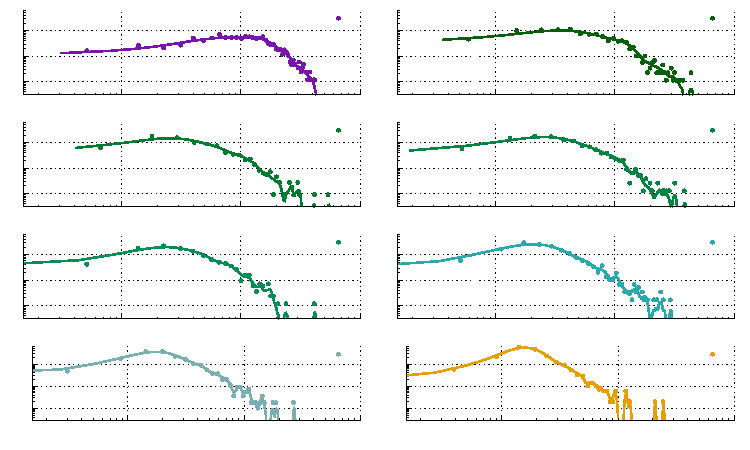
\includegraphics[width={360.00bp},height={216.00bp}]{figures/fig_MAD_binned_hump_pdf}}%
    \gplfronttext
  \end{picture}%
\endgroup
